% Z tego dokumentu renderujemy PDF z raportem z projektu. 

\documentclass{article}
\usepackage[utf8]{inputenc}

%\usepackage{graphicx} % jeśli z tego korzystam, to dodać ścieżkę do folderu z ilustracjami
% \graphicspath{ {folder_z_ilustracjami/} } % tu rzeczona ścieżka

% Poniżej wczytuję pakiet titling, który pozwala mi na dodanie podtytułu
% UWAGA: zainstalowałem ten pakiet w packages
\usepackage{titling}

\usepackage{graphicx} % grafika; ścieżka do wklejanych rysunków jest chyba domyślna i taka, jak folder tego dokumentu
\usepackage{hyperref} % hiperłącza

\usepackage{geometry} % do marginesów
\geometry{margin=1in} 

\usepackage[round]{natbib} % do wyświetlenia cytowania autor-rok

% Poniżej definiuję komendę \subtitle, która pozwala mi na dodanie podtytułu do mojego dokumentu
% UWAGA: newcommand świeci się na czerwno, bo to już istniejąca komenda latexa, którą tu nadpisuję
\newcommand{\subtitle}[1]{%
  \posttitle{%
    \par\end{center}
    \begin{center}\large#1\end{center}
    \vskip0.5em}%
}

\newcommand{\code}[1]{\texttt{#1}} % do kodu w tekście (inline)

\title{Sign Language Translator}
\subtitle{Introduction to Deep Learning for Natural Language Processing - Final Project Report}
\author{Wojciech Borysewicz}
\date{June 2026}

\begin{document}
\maketitle

\section{Introduction}
\label{sec:1}
\textbf{The project.} The project presented in this file is Sign Language Translator. It is a convolutional neural network-based model trained to 
recognize and classify American Sign Language (later: \textit{ASL}) gestures representing alphabetical letters (A–Z) and digits (0–9); 
the Translator is able to translate a given sequence of gesture images into a corresponding text string. The model was trained on a large dataset, 
consisting of more than 30 thousand ASL signs (numbers and letters).  
\newline

\noindent\textbf{About this file.} This file reports the experiments run as part of a final project for Deep Learning for Natural Language Processing classes. 
It will be joined with the Python script, where the experiments in question are run. Thus, this file also serves as a general description of 
the code as well as a manual to run the code and reproduce the results, if needed.  

The Python script, mentioned in the previous paragraph was written in the Google Collab environment and shall be refered to as the \textit{Google Collab notebook} 
or simply the \textit{Collab notebook}. This file's sections (or subsections) are named identically to the sections of the Collab notebook, which they
describe. Some of the Collab notebook's subsections are omitted in this report, if they do not contain any results (for example, metrics or statistics) 
or code, which would need to be discussed or presented in this document. This report is intended to describe the project and explain the decisions taken 
while writing the code, rather and pasting the code itself here. Should this report clarify the model's implementation insufficently, the Reader is asked to
look directly at the (extensively commented) code, present in the Google Collab notebook.  

This file is structured as follows. Section ~\ref{sec:2} describes the external Python libraries, which were used in the code, as well as other 
parameters (notably - frequently used constans), which were introduced to the experiments to make them more readable and more easily reproducible. 
Section ~\ref{sec:3} introduces and thoroughly describes the dataset, as well as Python code needed to load it into the Google Collab environment. 
Section ~\ref{sec:4} describes the machine learning models in use, as well as the functions needed to run the training pipeline. Section ~\ref{sec:5} makes the largest 
part of the report, as it describes the main part of the experiments. It is further divided into four subsections. In section ~\ref{sec:5.1} the chosen model's
architecture is described. In section ~\ref{sec:5.2}, the full training pipeline is described. Section ~\ref{sec:5.3} presents the model evaluation results. 
Finally, section ~\ref{sec:5.4} demonstartes the usage of the model (an example of ASL signs-to-text translation).

\section{Code running and instalation}
\label{sec:2}
The following Python (version 3.12.13) libraries were imported: Matplotlib (version 3.10.0), Numpy (version 2.0.2), Tensorflow (version 2.20.0), 
Pandas (2.2.2.). Modules os, random, math, itertools and pathlib from Python standard library were used as well. Also, particular methods from 
additional external libraries were in use: $\code{train\_test\_split}$ from SciKitLearn (version 1.6.1), and $\code{display}$ from IPython 
(version 7.34.0).  

Apart from importing the necessary modules and methods, several constants were added before the main code. Some of the constants, like $\code{TEST\_SIZE}$ 
were added to the code because they were used multiple times during the execution of various functions. Some of the other parameters were used 
far less frequently, but were introduced anyway in order to make the code more modular and easier to reproduce.
For example, introducing the constant $\code{FINAL\_RUNS}$ may seem unnecessary at the first glance (since it only stores an integer
and is used just once in the whole project), however, it makes clear the case of how many times the final model configuration is run (see 
$\code{average\_performance}$ method code in \textit{Model training and evaluation/Training and testing functions} section of the Google 
Collab notebook).

\section{Dataset}
\label{sec:3}
% Section contents - tutaj podać pochodzenie zbioru danych, najlepiej po prostu podlinkować artykuł lub chociaż podać tytuł i wymienić autorów.
% Opisać pokrótce ten zbiór danych zgodnie z tym, co w artykule i podlinkowanej w nim stronie.
The dataset used in this project was the American Sign Language Hand Gesture Image Dataset (later ASL-HG), prepared by a team of contributors lead by 
Md. Famidul Islam Pranto. The dataset was introduced and described in ~\citep{Pranto2026}. The dataset provides a comprehensive collection of exactly 
36,000 high resolution JPG images of ASL hand gestures across 36 classes (wchich yields 1000 images per class, thus making the dataset not only exceptionally
large, but also balanced). The colleccted images cover the full english alphabet (classes A-Z) as well as all digits (classes 0-9).  

The data were collected from 10 student volounteers in Mirpur, Dhaka, Bangladesh from May to June 2025. Each participant contributed 100 images per class; 
images were captured using smartphone HD cameras in various environments, making them highly diverse in lighting, background, viewing angles and distances 
as well as representative of different skin tones. Thus, the chosen dataset seemed to be the perfect choice for the Sign Language Translation.
In order to achieve this, the creators divided the dataset into two main parts (separate ZIP files): one containing the original unprocessed gesture images 
and the other one, containing the already processed images, divided into train/test splits (80\% training, 20\% testing) and standardized to a form suitable 
for immadiate model training. However, while this stands as a major advantage in virtually any machine learning task, I came to a conclusion that using the 
standard 80/20 split may be unnecessarily large for this task. Hence, I decided to try different train/test splits. Their values were stored in the 
$\code{TEST\_SPLITS}$ constant (Python list) in \textit{Reproducibility and configuration} part of the Google Collab notebook. The dataset splits 
were stratified, so class proportions were preserved in both training and test subsets.  

Since I decided to try other train/test splits from the usual 80/20 value, I needed to rejoin the initially separated \textit{train} and \textit{test} folders 
(from the subset of already processed images) in order for the whole collection of gesture images to be able to divide into desired splits. This is precisely what 
was done in the two code chunks under \textit{Path to Dataset (Google Drive)} and \textit{Loading the dataset} sections of the Google Collab notebook. All of 
the ASL-HG files were stored on a personal Google Drive. The dataset was loaded into the Collab notebook with a dedicated function from an $\code{Images\_Dataset}$
Python class, written especially for this project (for the full class code see \textit{Images Dataset class} section of the Collab notebook).  

It has to be reported that five images were not downloaded correctly (probably due to poor internet connection, Google Drive-related or
file-related issues): one of those images belonged to class \textit{Q}, and the four remaining images were part of a \textit{U} class. The issue
was not considered harmful for the project, since the remaining part of the dataset provided enough training material. Hence, there were 
no attempts to re-download the full dataset correclty.

The labels were encoded as one-hot vectors with 36 output dimensions, one for each gesture class. During training, a validation subset was created from the training
data using the $\code{validation\_split}$ argument. Therefore, the project used three effective subsets:

\begin{itemize}
  \item a training subset used to update model weights,
  \item a validation subset used to monitor training and select checkpoints,
  \item a test subset used for final evaluation
\end{itemize}  

The final split used in the selected model was 50/50 and the validation split was 10\% (that is: equal to $\code{VAL\_SPLIT}$ constant, set in the 
\textit{Reproducibility and configuration} section of the Google Collab notebook). The resulting numbers of training, validation and test examples were: 
16 197 training examples, 1 800 validation examples, 17 998 test examples. The final split was selected during the configuration search stage 
(described in section ~\ref{sec:4.2}). The class-level distribution is reported in table ~\ref{table:1}.

\section{Model training and evaluation}
\label{sec:4}
\subsection{Model (CNN) classes}
\label{sec:4.1}
The core model used in this project was a convolutional neural network implemented with TensorFlow/Keras. The model architecture was defined in a dedicated $\code{CNN\_Model}$ 
class. The class receives a list of convolutional and pooling layer configurations and builds a feature extractor consisting of repeated $\code{Conv2D}$ and $\code{MaxPooling2D}$ 
blocks. These layers are responsible for extracting spatial features from gesture images, such as hand contours, finger positions and local shape patterns. After the convolutional 
part, the model flattens the extracted feature maps and passes them through a dense classification head. The final layer uses the softmax activation function and returns a probability 
distribution over all 36 gesture classes.  

The class $\code{Convolutional\_Neural\_Network}$ acts as a wrapper around the CNN model. It stores the training data, builds the model, compiles it with the selected optimizer, 
trains it, and stores the training history. This wrapper also contains the plotting function used later to display loss and accuracy curves (in \textit{Plots} subsection of the 
\textit{Results} section of the Google Collab notebook). Thus, the CNN architecture is defined in one place, while the training and evaluation logic is handled separately.  

\subsection{Training and testing functions}
\label{sec:4.2}
The main function for training a single model configuration is $\code{run\_model}$. This function performs the complete workflow for one training run. It creates a train/test split, 
builds the CNN according to the selected architecture and hyperparameters, trains the model, saves the best validation checkpoint and evaluates the model on the test set. The function 
also returns the data split, the paths of images assigned to the training and test subsets, the training history, the trained network object, the final test metrics and the path to the 
saved weights. This is important because later parts of the project require not only a numerical score, but also access to the best run, the corresponding test split, and the saved weights.  

Model checkpointing was used during training in order to retrieve the best model run later (and use it as a selected model for the project's main purpose - ASL hand gesture translation). 
The checkpoint callback monitored the chosen validation metric, which was validation accuracy, and saved the model weights corresponding to the best validation performance. As a result, 
the evaluation can compare the model from the last epoch with the best saved checkpoint. The reported final score is based on the best checkpoint.  

The function $\code{average\_performance}$ is the main function of the final evaluation stage. After the optimal hyperparameter configuration has been selected (via the $\code{config\_search}$ 
function, described in the next paragraph), this function trains and evaluates that configuration several times using different random seeds (the seeds which were used were stored in the $\code{SEEDS}$ list, set at 
the beginning of the Google Collab notebook, along with other important constants and parameters). Each run uses the same train/test ratio but a different random split and model initialization. 
In the code, the final model configuration is run exaclty 5 times. The best, mean and standard deviation of accuracy are returned by the function. Their values, achieved
by the final model in this project are reported in section ~\ref{sec:5.3}.

As suggested above, this project included a configuration search step. Its goal was to compare different CNN and training hyperparameter settings before selecting the optimal hyperparameter configuration. 
The search space included the CNN architecture, learning rate, batch size, dense layer size, dropout rate, image size and train/test split ratio. The configuration search is performed by the 
$\code{config\_search}$ function. This method first utilizes the helper function $\code{sample\_configuration}$, which randomly selectes a fixed number of configurations from the full hyperparameter grid 
(avoiding testing every possible combination). Then, the $\code{config\_search}$ function trains one model for each sampled configuration. Each configuration is trained for a limied number of epochs and 
evaluated using validation performance. The selected score is based on the best validation metric obtained during training.  

The best configuration selected by configuration search consisted of the $\code{large}$ achitecture (see section ~\ref{sec:5.1}) and the following parameters: 
$\code{learning\_rate} = 0.001$, $\code{batch\_size}=16$, $\code{dense\_units}=64$, $\code{dropout\_rate}=0.3$, $\code{img\_size}=(64,64)$, $\code{test\_size}=0.5$.  

\section{Main}
\label{sec:5}
\subsection{Model architecture (layers)}
\label{sec:5.1}
The final model was a convolutional neural network for 36-class image classification. The input to the model was a grayscale image resized $64 \times 64$ pixels. The final architecture was the $\code{large}$
architecture, consisting of four convolutional blocks. Each block contains one Conv2D layer followed by one MaxPooling2D layer. The number of convolutional filters increases across the network, allowing the 
model to learn progressively more complex image features. The early layers detect simple local patterns, while deeper layers can represent more abstract hand-shape features. After the convolutional feature 
extractor, the output is flattened and passed through a dense classification head with dropout regularization and a final softmax layer over 36 gesture classes (to see the exact $\code{large}$ architecture 
implementation, as well as other tested architectures and their implementation go to \textit{Model architecture (layers)} section of the Google Collab notebook).

\subsection{Train, test and evaluate models}
\label{sec:5.2}
This section presents the full training pipeline. It consisted of the following stages.  

First, the dataset was loaded from the processed ASL-HG folders (see section ~\ref{sec:3}). Second, upon loading the dataset, all images were vectorized into numerical arrays. Each image was loaded in grayscale, 
resized to the selected image size, normalized to the $\code{([0,1])}$ range and reshaped to include a single channel dimension. Labels were converted into one-hot vectors. Third, configuration search was 
performed. Fourth, the selected, optimal configuration was evaluated repeatedly using the $\code{average\_performance}$ function. Finally, the best final run was selected. Its saved weights were used to 
reconstruct the final model for the breakdown table and the ASL signs-to-gesture translation.

After the repeated final evaluaton, the best final run was selected. The corresponding path to saved weights was stored and used to reconstruct the final CNN model.
This reconstructed model is referred to as the \textit{final model} or the \textit{selected model} in this report.  

The seed of the best final run was also stored. This made it possible to recreate the exact train/test split used by that run and to ensure that the images used in 
the final demonstration came from the test subset rather than from the training subset (see \textit{Final model} subsesction of \textit{Main} section of the Google
Collab notebook). 

\subsection{Results}
\label{sec:5.3}
The final repeated evaluation of the selected model (carried out by the $\code{average\_performance}$ function) produced the following summary:

\begin{itemize}
  \item best accuracy: 0.9998,
  \item mean accuracy: 0.9993,
  \item SD of accuracy: 0.0005
\end{itemize} 

Table ~\ref{table:1} - created with a dedicated $\code{make\_breakdown\_table}$ method (see \textit{Breakdown table function}) 
subsection of \textit{Model training and evaluation} section of the Google Collab notebook - shows class-level test performance achieved by 
the selected model during the best final run. As the table shows, model's results are either perfect or near-ceilling, indicating that the 
classifier performs both excellent and consistently across the 36 hand gesture categories; only two minor differences between labels can be observed 
(for \textit{H} and \textit{W} classes). Thus, the overall pattern suggests that no single class was systematically misclassified more often 
than the others. Therefore, the selected CNN architecture appears to be suitable for the final gesture-to-text translation.
Figure ~\ref{fig:1} shows the learning curves of the final model, including training and validation loss and accuracy over epochs. 
The curves were obtained by re-running the selected model configuration with the same seed as the best final run (see \textit{Saving the best run} 
in \textit{Final model} subsection of \textit{Main} section of the Google Collab notebook). The plots show that training and validation accuracy
increase over epochs, while training and validation loss decrease over epochs and then stabilize. The validation curves follow the training curves
closely, which suggests that the model generalizes well to unseen data. Thus, the plots indicate, that the model was learning effectively and report 
no clear signs of overfitting or underfitting. 

\begin{center}
  \begin{table}[ht]
    \begin{tabular}{|c |c |c |c |c |c|}
      \hline
      Label & Total data & Training data & Test data & Correct predictions & Accuracy \\
      \hline
      0 & 1000 & 500 & 500 & 500 & 1.0000 \\
      
      1 & 1000 & 500 & 500 & 500 & 1.0000 \\
      
      2 & 1000 & 500 & 500 & 500 & 1.0000 \\
      
      3 & 1000 & 500 & 500 & 500 & 1.0000 \\
      
      4 & 1000 & 500 & 500 & 500 & 1.0000 \\
      
      5 & 1000 & 500 & 500 & 500 & 1.0000 \\
      
      6 & 1000 & 500 & 500 & 500 & 1.0000 \\
      
      7 & 1000 & 500 & 500 & 500 & 1.0000 \\
      
      8 & 1000 & 500 & 500 & 500 & 1.0000 \\
      
      9 & 1000 & 500 & 500 & 500 & 1.0000 \\
      
      A & 1000 & 500 & 500 & 500 & 1.0000 \\
      
      B & 1000 & 500 & 500 & 500 & 1.0000 \\
      
      C & 1000 & 500 & 500 & 500 & 1.0000 \\
      
      D & 1000 & 500 & 500 & 500 & 1.0000 \\
      
      E & 1000 & 500 & 500 & 500 & 1.0000 \\
      
      F & 1000 & 500 & 500 & 500 & 1.0000 \\
      
      G & 1000 & 500 & 500 & 500 & 1.0000 \\
      
      H & 1000 & 500 & 500 & 498 & 0.9960 \\
      
      I & 1000 & 500 & 500 & 500 & 1.0000 \\
      
      J & 1000 & 500 & 500 & 500 & 1.0000 \\
      
      K & 1000 & 500 & 500 & 500 & 1.0000 \\
      
      L & 1000 & 500 & 500 & 500 & 1.0000 \\
      
      M & 1000 & 500 & 500 & 500 & 1.0000 \\
      
      N & 1000 & 500 & 500 & 500 & 1.0000 \\
      
      O & 1000 & 500 & 500 & 500 & 1.0000 \\
      
      P & 1000 & 500 & 500 & 500 & 1.0000 \\
      
      Q & 999 & 499 & 500 & 500 & 1.0000 \\
      
      R & 1000 & 500 & 500 & 500 & 1.0000 \\
      
      S & 1000 & 500 & 500 & 500 & 1.0000 \\
      
      T & 1000 & 500 & 500 & 500 & 1.0000 \\
      
      U & 996 & 498 & 498 & 498 & 1.0000 \\
      
      V & 1000 & 500 & 500 & 500 & 1.0000 \\
      
      W & 1000 & 500 & 500 & 499 & 0.9980 \\
      
      X & 1000 & 500 & 500 & 500 & 1.0000 \\
      
      Y & 1000 & 500 & 500 & 500 & 1.0000 \\
      
      Z & 1000 & 500 & 500 & 500 & 1.0000 \\
      \hline
    \end{tabular}
    \caption{The breakdown table, showing the final model's accuracy by class, which is the number of correctly predicted test examples belonging to a certain class 
    (\textit{correct predictions} value) dividied by the total number of test datapoints from that class (\textit{test data}) value.}
    \label{table:1}
  \end{table}
\end{center}

\begin{figure}[ht]
  \centering
  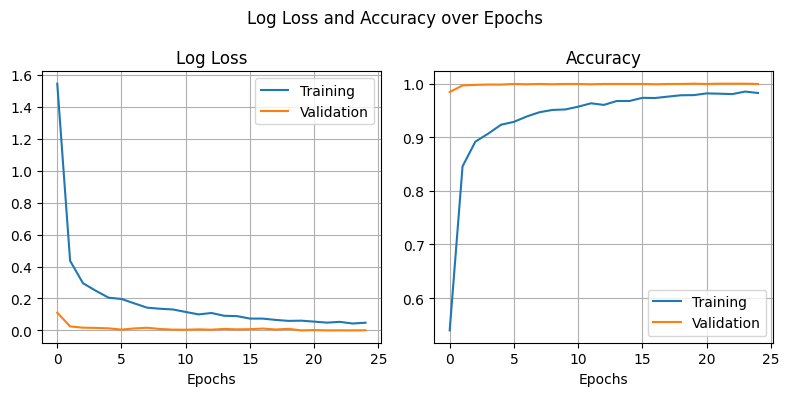
\includegraphics[scale=0.75]{images/report_plots.png}
  \caption{The training curves: training logarithmic loss, validation logarithmic loss, training accuracy and validation
  accuracy over epochs.}
  \label{fig:1}
\end{figure}

\subsection{Sign language translation}
\label{sec:5.4}
This section reports the final part of the project - performing the image-to-text translation task. This was done with a $\code{translate\_gesture\_sequence}$ function. 
This method receives a sequence of image paths and and uses two helper functions, $\code{preprocess\_single\_image}$ and $\code{predict\_single\_gesture}$, to 
preprocess and classify each image. Each image is preprocessed in the same way as the images used during model training. After preprocessing, each image is passed 
independently through the final model. The model returns a softmax output vector over all gesture classes. The class with the highest softmax value is selected as the 
predicted label for that image. The $\code{translate\_gesture\_sequence}$ function stores the predicted labels in their original order and concatenates them into a 
single text string. Thus, it performs a sequence of independent single-image classifications and then joins the predicted class labels into the final predicted text.
In addition to the predicted text, the function returns a prediction table. This table contains one row for each input image. The $\code{predicted\_label}$ column 
reports the class selected by the model, while the $\code{predicted\_class\_probability}$ column reports the softmax value assigned to that selected class. 
This value can be interpreted as the model's confidence score for its own prediction.

Model's translating ability was demonstrated using three trials. First, the model had to translate a sequence of three manually selected images,
correspoding to the text "ASL". Second, model had to translate a sequence of four manually selected images, corresponding to 
the number 2026. For the third demonstartion, five images (either letter or number hand gestures) were sampled randomly from the test subset. 
Their true labels were read from the folder names and compared with the predicted labels. The random sequence was "F9423".
The image sequences used in trials number one, two and three are shown in figures 2, 3, 4, respectively.

\begin{figure}[ht]
  \centering
  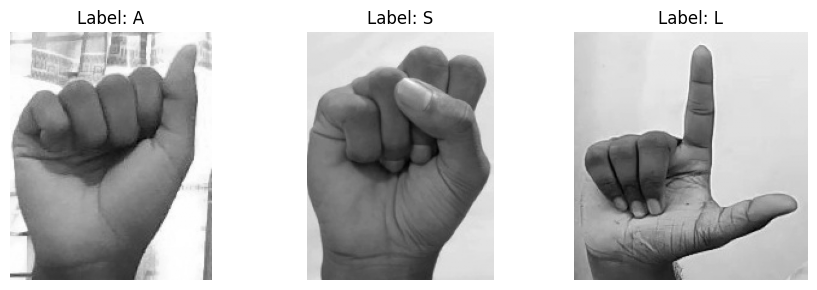
\includegraphics[scale=0.7]{images/ex01_signs.png}
  \caption{The sequence of three hand gestures model had to translate into text as part of the first trial. Those images were
  selected manually and they represented the text "ASL", an abbreviation of "American Sign Language".}
  \label{fig:2}
\end{figure}

\begin{figure}[ht]
  \centering
  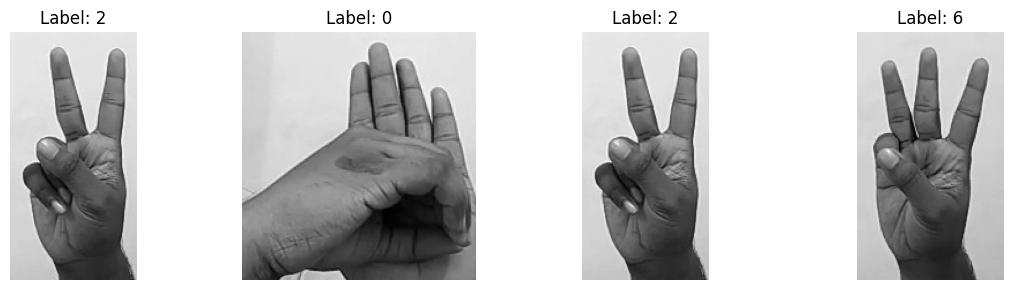
\includegraphics[scale=0.6]{images/ex02_signs.png}
  \caption{The sequence of four hand gestures model had to translate into text as part of the second trial. Those images were
  selected manually and they represented the number 2026, refering to the current year.}
  \label{fig:3}
\end{figure}

\begin{figure}[ht]
  \centering
  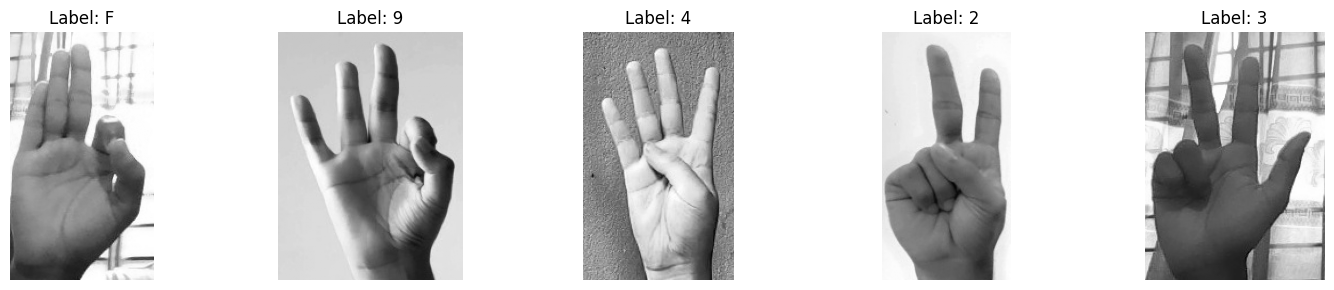
\includegraphics[width=0.95\textwidth,scale=0.6]{images/ex03_signs.png}
  \caption{The sequence of five hand gestures model had to translate into text as part of the third trial. Those images were
  selected randomly and they do not represent any meaningful text.}
  \label{fig:4}
\end{figure}

In each case, the model correclty translated every sequence of images into text. The $\code{predicted\_class\_probability}$ values, always very 
close or equal to $1$ also indicate, that the model assigned its predictions with high confidence. Those values, achieved in the first, second and
the third trials are presented in tables ~\ref{table:2}, ~\ref{table:3}., ~\ref{table:4}, respectively. Overall, the translation demonstration 
confirmes, that the trained classifier works well and can be used as a simple image-to-text translator.

\begin{center}
  \begin{table}[ht]
    \begin{tabular}{|c |c |c |c|}
      \hline
      Position & Predicted label & Predicted class probability \\
      \hline
      1 & A & 0.999815 \\
      2 & S & 0.994501 \\
      3 & L & 1.000000 \\
      \hline
    \end{tabular}
    \caption{A table returned by the $\code{translate\_gesture\_sequence}$ after the first performed translation. This table was returned alongside
    the expected text and the one predicted by the model - which, in both cases, was "ASL".}
    \label{table:2}
  \end{table}
\end{center}

\begin{center}
  \begin{table}[ht]
    \begin{tabular}{|c |c |c |c|}
      \hline
      Position & Predicted label & Predicted class probability \\
      \hline
      1 & 2 & 0.997431 \\
      2 & 0 & 1.000000 \\
      3 & 2 & 0.997431 \\
      4 & 6 & 1.000000 \\
      \hline
    \end{tabular}
    \caption{A table returned by the $\code{translate\_gesture\_sequence}$ after the second performed translation. This table was returned alongside
    the expected text and the one predicted by the model - which, in both cases, was "2026".}
    \label{table:3}
  \end{table}
\end{center}

\begin{center}
  \begin{table}[ht]
    \begin{tabular}{|c |c |c |c|}
      \hline
      Position & Predicted label & Predicted class probability \\
      \hline
      1 & F & 0.999992 \\
      2 & 9 & 0.973571 \\
      3 & 4 & 0.999917 \\
      4 & 2 & 0.952181 \\
      5 & 3 & 1.000000 \\
      \hline
    \end{tabular}
    \caption{A table returned by the $\code{translate\_gesture\_sequence}$ after the second performed translation. This table was returned alongside
    the expected text and the one predicted by the model - which, in both cases, was "F9423".}
    \label{table:4}
  \end{table}
\end{center}

\clearpage
\renewcommand{\refname}{Sources}
\bibliographystyle{plainnat}
\bibliography{DL_report_bibliography}

\end{document}
